% !TEX root =  ../FinalReport.tex

\chapter{Design}
\label{sec:Design} 

\section{Command-Line Interface}
The compiled binary uses a command-line interface to configure and run one of many subcommands available.
These subcommands are:\label{sec:DesignSubcommands}
\begin{itemize}
    \item \texttt{makeinput}, which generates simulation input files, fulfilling \cref{req:GenerateState}.
    \item \texttt{fixedtime}, which runs a headless simulation for a fixed time, fulfilling \cref{req:HeadlessSim}.
    \item \texttt{compare}, which compares two simulation states for equality, fulfilling \cref{req:Compare}.
    \item \texttt{renderppm}, which visualizes a simulation state in the same way the original ACA coursework did.
    \item \texttt{convert2newbinary}, for converting ACA simulation state files to a potential new format (see \cref{sec:FileFormat}). Currently a no-op.
    \item \texttt{run}, which starts a real-time visualized simulation, fulfilling \cref{req:VizSim}.
\end{itemize}
Splitting the program into subcommands was inspired by Git\cite{tool:Git}, and avoids creating separate binaries for each operation.
Each subcommand can be configured with command-line options conforming to POSIX standard\cite{IEEE2018UtilityConventions}.
Examples of using the program are in \cref{fig:BashExampleUsage}.
\begin{figure}[ht]
    \centering
    \begin{lstlisting}[language=bash]
# Create an input file based on simple_layout with a size of 1x2 metres
./sim_cuda makeinput ./simple_layout.png 1 2 ./initial.bin

# Run it in headless mode for 10 seconds
./sim_cuda fixedtime --backend=cuda ./fluid.json ./initial.bin 10 \
                        -o ./output_after_10.bin

# Compare it to the expected output
./sim_cuda compare ./output_after_10.bin ./expected_after_10.bin

# Render it out to an image
./sim_cuda renderppm ./output_after_10.bin zeta ./output_after_10.ppm

# Try visualizing it in real-time
./sim_cuda run --backend=cuda ./fluid.json ./initial.bin
\end{lstlisting}
    \caption{Example usage of the simulation program}
    \label{fig:BashExampleUsage}
\end{figure}

\section{Generating Inputs}
The \texttt{makeinput} subcommand allows input simulation states to be generated from image files.
Each pixel of the input image represents a cell of the grid, including padding cells\footnote{This can allow the padding cells to be fluids rather than boundaries, which is incorrect. In the future this will be changed to add padding cells once the image is parsed.}, where non-black pixels are denoted as boundary cells and are fluid cells otherwise.
The example in \cref{fig:ExampleMakeinput} shows an example file which creates a rectangular obstacle, and the visualization of the generated state.
\begin{figure}[ht]
    \centering

    \subcaptionbox{Base Image%
    }[\linewidth]{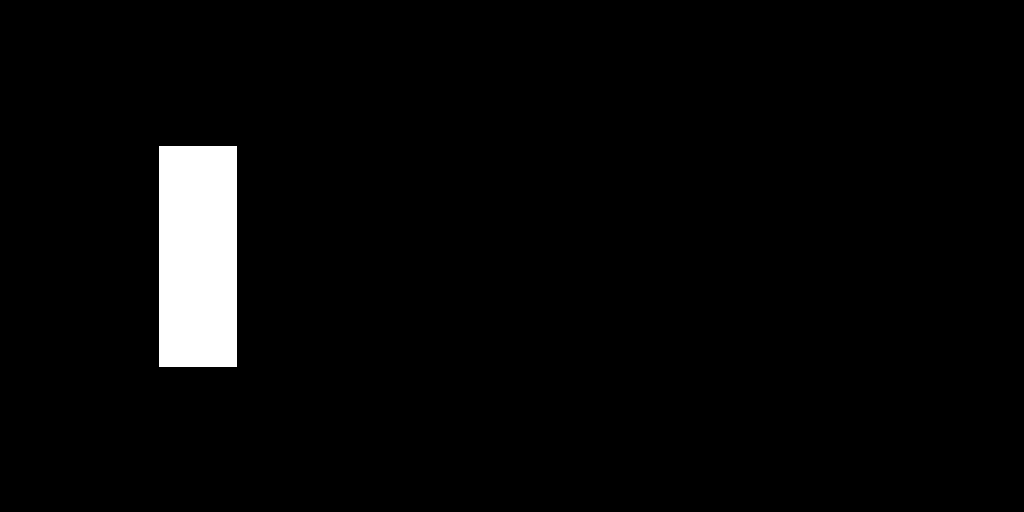
\includegraphics[]{Ch42Design/figures/simple_layout.png}
    }
    
    \subcaptionbox{Simulation%
    }[\linewidth]{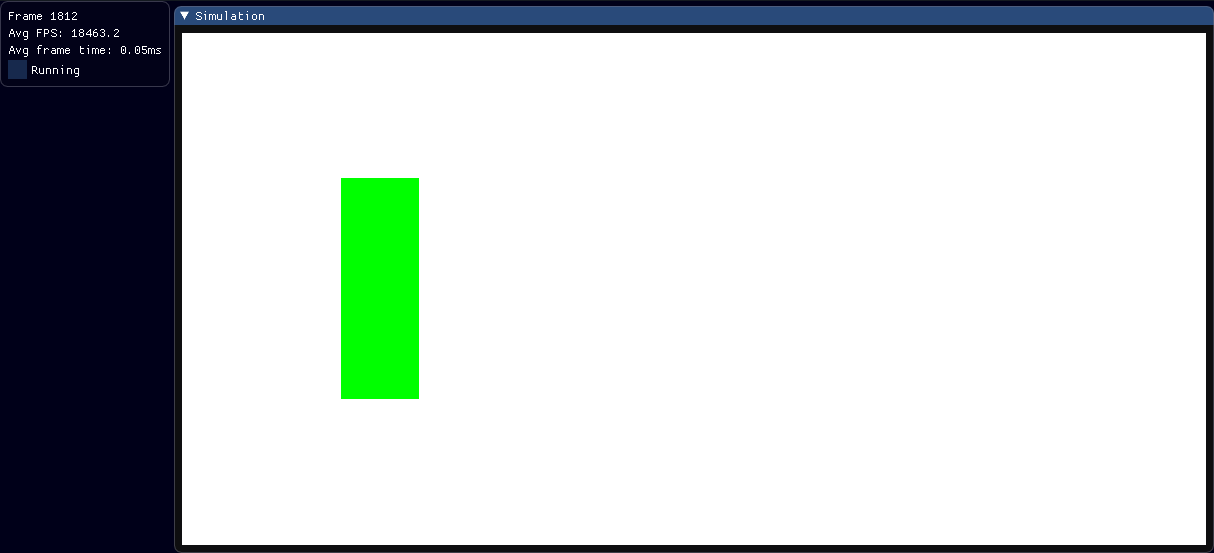
\includegraphics[width=0.5\linewidth]{Ch42Design/figures/example_sim_of_simple_layout.png}
    }
    
    \caption{Example conversion of an image to a simulation state}
    \label{fig:ExampleMakeinput}
\end{figure}

Velocities and pressure in every cell are currently set to constant default values.
For velocities, this is \SI{1}{m/s} east, equal to the default flow of incoming fluid, which may cause issues with correctness.
An example would be a situation where fluid is occluded from the input direction by an obstacle, but moves east anyway with no reason to do so.
%it would not be correct for that fluid to move) 
This will likely be changed to zero out initial velocity, requiring some simulation to take place before the fluid begins to move.

The exact initial value of pressure is inconsequential as the simulation only cares about the difference between cells.
This means the only significant point is that the pressure is equal over all cells, so the system should be in equilibrium.
This may be inconsistent with the nonzero velocities mentioned above, which is another reason to zero them out instead.


\section{File Formats}
\label{sec:FileFormat}
To fulfil \cref{req:StoreState} two file formats have been defined to store simulation data and parameters.

\subsection{Fluid Parameters}
Parameters that are characteristic of a particular fluid or simulation type are stored in a ``Fluid Parameters'' file.
This includes the Reynolds number, the timestep safety factor, and the maximum iteration count for the Poisson solver.
They are stored in a JSON format to be human-readable, are reusable for different simulation states, and can be easily edited by the end user.
An example is shown in \cref{fig:FluidParamsExample}.

\begin{figure}[ht]
% \begin{wrapfigure}{r}{0.5\textwidth}
    \centering
    %\begin{minted}{json}
    \begin{lstlisting}[language=JSON]
{
    "Re": 150.0,
    "initial_velocity_x": 1.0,
    "initial_velocity_y": 0.0,
    "timestep_divisor": 60,
    "max_timestep_divisor": 480,
    "timestep_safety": 0.5,
    "gamma": 0.9,
    "poisson_max_iterations": 100,
    "poisson_error_threshold": 0.001,
    "poisson_omega": 1.7
}
\end{lstlisting}
% \end{minted}
    \caption{An example Fluid Parameters file.}
    \label{fig:FluidParamsExample}
% \end{wrapfigure}
\end{figure}

\subsection{Simulation State}
Data unique to an individual state such as simulation resolution, physical size, and velocity fields are stored in a binary format reused from the ACA project.
As the data is much more sensitive to individual modifications\footnote{i.e. changing a single value in the velocity field can introduce discontinuities}, it makes more sense to store this data in a binary format where it cannot be easily modified by a user.
Additionally the binary format is much smaller than any text-based format, which helps as the volume of data stored is much larger than that stored in the fluid parameters.


% \begin{figure}[ht]
    \centering
    \todomark{This will be a small diagram of the file format, which might be dropped for the Progress report if it takes too much time}
    \caption{A visual representation of the binary file format.}
    \label{fig:BinaryFileFormat}
\end{figure}
% The structure of the binary format is shown in \cref{fig:BinaryFileFormat}.
There is no magic string at the start of the file, which may be introduced in a new version.
The header consists of a pair of unsigned 32-bit integers specifying the resolution of the simulation, and a pair of 32-bit floating point numbers specifying the physical dimensions of the simulation.
From there, four sets of data for each column are stored, including the boundary padding squares:
\begin{enumerate}
    \item Horizontal Velocity $u$ (\texttt{float32})
    \item Vertical Velocity $v$ (\texttt{float32})
    \item Pressure $p$ (\texttt{float32})
    \item Cell Flags, defining which adjacent squares are boundaries (\texttt{uint8})
\end{enumerate}
This structure is somewhat unintuitive and error-prone, an example being the Cell Flags which may end up being inconsistent between adjacent cells, but for the sake of compatibility with ACA data it has been kept.
In the future it may be updated to a safer format.

\section{Simulation Backends}
To allow easy comparisons between CPU and GPU simulations the program contains multiple simulation backends which can be requested when running a headless simulation\footnote{The realtime visualization currently only supports the CUDA-based backend, violating \cref{req:GPUCapable}.}.
The headless simulation uses a \texttt{--backend} command line option to allow the user to choose the backend from this selection:\label{sec:DesignBackends}
\begin{itemize}
    \item Null, a backend which does no simulation for testing purposes.
    \item CPU Simple, equivalent to pre-optimization ACA code.
    \item CPU Optimized, equivalent to the submission for ACA, bit-equivalent to CPU Simple.
    \item CPU Optimized Adapted, a version of CPU Optimized slightly modified to be closer to the GPU version.
    \item CUDA Backend V1, the only GPU-based backend.
\end{itemize}

Currently the only modification present in the CPU Optimized Adapted backend is the removal of double-precision floating point logic, which is not present on the GPU for speed concerns.
However once the GPU introduces residual checking for the iterative solver, or any other major changes to the pipeline, they will be introduced into this backend to ensure a like-for-like comparison.

\section{Visualization Pipeline}
This section details the extra code implemented in order to efficiently and effectively visualize simulation results in real time.
This is not related to the \texttt{renderppm} subcommand, which uses CPU code to render a single simulation state as an image.

\subsection{Work Scheduling}
The most important tasks are run on the GPU, and are the limiting factor for performance.
This means it's important that the GPU is running at all times.
Points where the GPU is doing no useful work are known as ``bubbles''.
% \todopending{Add figures with first 2 examples of pipeline bubbles vs. no pipeline bubbles}

To avoid these bubbles a GUI thread is spawned to prepare the current frame's draw commands and handle user input.
This runs in parallel with the simulation thread, which dispatches CUDA kernels for the simulation tick(s).
Once the sim is finished, it waits on the GUI thread (which should always be done by this point) and dispatches the draw commands through Vulkan.
It then dispatches the GUI thread again, waits for the render to finish and then immediately starts the next simulation.

\Cref{fig:CurrentSwimlane} shows the scheduling in more detail.
The GUI work can execute anywhere within the dashed lines and still not delay the final draw.
Note that the GPU is always doing useful work, and there are no bubbles.
\begin{figure}[ht]
    \centering
    \centerline{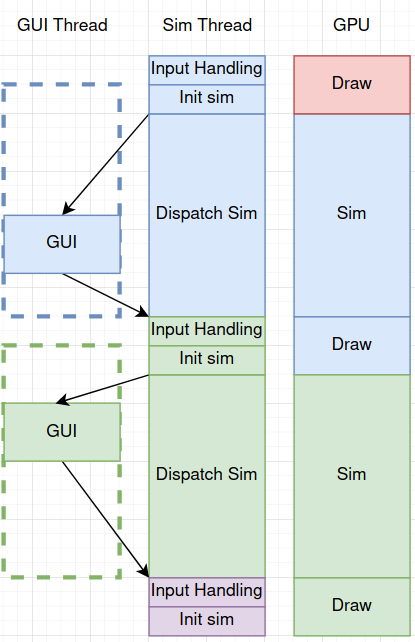
\includegraphics[width=0.5\linewidth]{ProgressReport/Ch42Design/figures/threading_usage_2.png}}
    \caption{Thread utilization diagram.}
    \label{fig:CurrentSwimlane}
    % \caption*{The GUI thread can execute anywhere within the dashed lines and still be on time.}
\end{figure}


Currently it is assumed that the rendering of one frame and the simulation of the next frame cannot happen in parallel.
\label{sec:DesignBetterScheduling}
This is also enforced by the fact that velocity and pressure buffers are used by both the simulation and the render, meaning that a simulation could not update those buffers without invoking a race condition.
However if the GPU has spare cores available while rendering a frame, then the simulation could use these cores on the next simulation at the same time.
Furthermore, most of the simulation can take place without writing to the velocity and pressure buffers, so those parts of the simulation could be run in parallel with the rendering without any worries.
Or, of course, the simulation could be double-buffered and run entirely in parallel with the rendering.

\subsection{Simulation Timing}
% \todopending{This is probably too complicated to get into fully right now. Wait until full report?}
% Define terminology: simulation time, simulation tick, real time, frame number 

% Currently the code simulates 16ms of simulation time every frame, regardless of how long it actually takes to do so.
As specified by \cref{req:VizSomeSpeed} there are two acceptable modes that the visualization can run in:
Flat Out (\cref{req:VizFlatOut}), where the simulation runs as fast as possible;
and Locked Framerate (\cref{req:VizLockedFPS}), where a frame-rate is selected and the visualization only produces that many frames per second.
The definition of a flat-out speed is that if Frame $N$ takes some amount of real-world time $t_N$, then the next frame should simulate $t_N$ seconds of simulation-time before it is presented.
This way the simulation runs as fast as possible, but it could lead to situations where if the simulation takes too long, the next simulation will have to simulate even more time and take longer etc.

With a locked frame-rate the simulation selects a timestep $\delta{t}$ to simulate for each frame, and limits the speed at which frames are produced.
If the frame-rate is 60 frames per second, then the visualization would potentially have to delay itself so that each frame takes $1/60 = \SI{16.67}{ms}$.

Currently the visualization does not take either of these approaches, but simulates a fixed $\delta{t} = 1/60$ without limiting the frame-rate.
This means on the researcher's current setup, which has a monitor capable of showing 120fps, the visualization runs 120 ticks per second which results in a simulation that's 2x faster than real-time.
This shows the simulation is fast, which is promising, but it fails the requirements.

\section{Comparison Heuristics}
In the comparison subcommand heuristics are used to judge if one simulation is accurate and precise with respect to the other.
This does not quite fulfil \cref{req:CompareBinary}, as there are two results and two heuristics used instead of just one.
To fix this, it is planned that the comparison will produce \texttt{SIMILAR} if the simulations are both accurate and precise, and \texttt{NOT~SIMILAR} otherwise.
The program may then provide additional information to help the user determine the cause of the problem.

This assumes one of the supplied states is a known-valid simulation state, and the other is not.
Two simulation state files are provided, and the velocity and pressure values $u, v, p$ are compared separately.
The simulation states must be of the same resolution, and should use the same boundary squares (although this is not currently checked).

The comparison is performed by calculating the mean and standard deviation of the square error between the datasets.
These are then compared to tolerance values to produce two binary outputs: ACCURATE if the mean is below tolerance, and PRECISE if the standard deviation is below tolerance.
Examples are shown in \cref{fig:example_comparisons}.

The tolerance for the mean was derived from an expected error magnitude of $\pm 10^{-7}$, which was squared to produce $10^{-14}$.
It is assumed that the standard deviation should always be smaller than the mean, so the tolerance for standard deviation is also $10^{-14}$.
\todopending{More examination of this? Square error always >0 => if std.dev > mean then distribution cannot be normal? Prob wait for full report}

\begin{figure}[ht]
    \centering
    \begin{center}
    \lstset{language=bash,
    numbers=none,
    keywordstyle=[2]\color{red},
    keywords=[2]{INACCURATE,IMPRECISE},
    keywordstyle=[3]\color{green},
    keywords=[3]{ACCURATE,PRECISE}
    }
    % \lstset{language=bash,
    % linewidth=0.5\linewidth
    % % keywordstyle=[2]\color{red},
    % % keywords=[2]{INACCURATE,IMPRECISE},
    % % keywordstyle=[3]\color{green},
    % % keywords=[3]{ACCURATE,PRECISE}
    % }
    % \subcaptionbox{Comparison of equal states}[0.5\linewidth]{\begin{frame}[fragile]\end{frame}}
    %[xleftmargin=-0.2\textwidth]
\begin{subfigure}{0.4\textwidth}\begin{lstlisting}
Velocity X:
    Sq. Error Mean:     0     ACCURATE
    Sq. Error Std. Dev: 0     PRECISE
Velocity Y:
    Sq. Error Mean:     0     ACCURATE
    Sq. Error Std. Dev: 0     PRECISE
Pressure:
    Sq. Error Mean:     0     ACCURATE
    Sq. Error Std. Dev: 0     PRECISE\end{lstlisting}%
    \caption{Comparison of Equal States}%
\end{subfigure}%
\hspace{0.02\textwidth}
\begin{subfigure}{0.5\textwidth}\begin{lstlisting}[]
Velocity X:
    Sq. Error Mean:     0.0233842     INACCURATE
    Sq. Error Std. Dev: 0.0996487     IMPRECISE
Velocity Y:
    Sq. Error Mean:     0.00566354    INACCURATE
    Sq. Error Std. Dev: 0.0139529     IMPRECISE
Pressure:
    Sq. Error Mean:     0.0214799     INACCURATE
    Sq. Error Std. Dev: 0.0511252     IMPRECISE\end{lstlisting}%
\caption{Comparison of Unequal States}%
\end{subfigure}
\end{center}
% Velocity X:
%         Sq. Error Mean:                   0     ACCURATE
%         Sq. Error Std. Dev:               0     PRECISE
% Velocity Y:
%         Sq. Error Mean:                   0     ACCURATE
%         Sq. Error Std. Dev:               0     PRECISE
% Pressure:
%         Sq. Error Mean:                   0     ACCURATE
%         Sq. Error Std. Dev:               0     PRECISE
    
%     \subcaptionbox{Comparison of unequal states%
%     }[0.5\linewidth]{\begin{lstlisting}
% Velocity X:
%         Sq. Error Mean:           0.0233842     INACCURATE
%         Sq. Error Std. Dev:       0.0996487     IMPRECISE
% Velocity Y:
%         Sq. Error Mean:          0.00566354     INACCURATE
%         Sq. Error Std. Dev:       0.0139529     IMPRECISE
% Pressure:
%         Sq. Error Mean:           0.0214799     INACCURATE
%         Sq. Error Std. Dev:       0.0511252     IMPRECISE
% \end{lstlisting}}
    
    \caption{Examples outputs from the comparison tool.}
    \label{fig:example_comparisons}
\end{figure}